%\documentclass[letterpaper,draft]{beamer}
\documentclass[letterpaper,handout, mathserif]{beamer}
%\documentclass[letterpaper]{beamer}

%---multiple pages on one sheet, ADD for handout--
%\usepackage{pgfpages}
%\pgfpagesuselayout{4 on 1}[letterpaper, landscape, border shrink=1mm]
%-------------------------------------------------
\usepackage{amsmath,amsfonts}
%\usepackage{booktabs}
%\usepackage{mdwlist}
\usepackage{amsfonts}
%\usetheme{Copenhagen}
%\usetheme{warsaw}
\setbeamertemplate{navigation symbols}{}
\usepackage[english]{babel}
\def\ul{\underline}
% or whatever

\usepackage[latin1]{inputenc}
\subject{Talks}

\def\Sum{\sum\nolimits}
\def\Prod{\prod\nolimits}
\def\p{\mathrm P}
\def\E{\mathbb E}
\def\V{\mathrm Var}
\def\CV{\mathrm Cov}
\def\X{\mathcal{X}}
\def\dt{\Delta}
\def\typo#1{\alert{#1}}
%-------------Answers------------
\def\Hide#1#2{\ul{~~~\onslide<#1>{\alert{#2}}~~~}}
\def\hide#1#2{\ul{~~\onslide<#1>{\alert{#2}}~~}}
\def\hid#1#2{\onslide<#1>{\alert{#2}}}
%------Centered Page Number------
\defbeamertemplate{footline}{centered page number}
{%
  \hspace*{\fill}%
  %\usebeamercolor[fg]{page number in head/foot}%
  %\usebeamerfont{page number in head/foot}%
  \small Lecture \chapnum\ - \insertframenumber%
  \hspace*{\fill}\vskip2pt%
}

%\usepackage{tikz}
%\usebackgroundtemplate{%
%\tikz\node[opacity=0.3] {\includegraphics[height=\paperheight,widht=\paperwidth]{ctanlion}};}

%\usebackgroundtemplate{%
%  %\rule{0pt}{\paperheight}%
%  \parbox[c][\paperheight][c]{\paperwidth}{\centering\includegraphics[width=.65\paperwidth]{UClogo.pdf}}
%  %\hspace*{\paperwidth}
%}

\def\chapnum{17}
%--------------------------------
\setbeamertemplate{footline}[centered page number]

\title{STAT253/317 Lecture \chapnum} \date{} \author{Cong Ma}
\begin{document}
% ----------------------------------------------------------------------
\begin{frame}
\maketitle
\begin{center}\large
\begin{tabular}{ll}
7.4 & Renewal Reward Processes\\
7.5.1 & Alternating Renewal Processes
\end{tabular}
\end{center}
\end{frame}
% ----------------------------------------------------------------------
\begin{frame}{7.4~ Renewal Reward Processes}
Let $\{N(t),t\ge 0\}$ be a renewal process with i.i.d. interarrival times
$\{X_i, i\ge 1\}$. Let $R_i$, $i = 1,2,\ldots$ be i.i.d random variables. $R_i$
may depend on the $i$th interarrival time $X_i$, but $(X_i,R_i)$ are i.i.d.
random variable pairs. The compound process
$$
R(t) = \Sum_{i=1}^{N(t)}R_i
$$
is called a \structure{\em renewal reward process}. $R_i$ may be considered as \structure{\em reward}
earned during the $i$th cycle, and $R(t)$ represents the total reward
earned up to time $t$.\bigskip

{\bf Proposition 7.3} If $\E[R_1] < \infty$ and $\E[X_1] < \infty$, then
\begin{itemize}
\item[(a)] $\displaystyle\lim_{t\to\infty}\dfrac{R(t)}{t}=\dfrac{\E[R_1]}{\E[X_1]}$ with probability 1
\item[(b)] $\displaystyle\lim_{t\to\infty}\dfrac{\E[R(t)]}{t}=\dfrac{\E[R_1]}{\E[X_1]}$
\end{itemize}
\end{frame}
% ----------------------------------------------------------------------
\begin{frame}{Proof of Proposition 7.3(a)}
We give the proof for (a) only. To prove this, write
$$\frac{R(t)}{t}=\frac{\Sum_{i=1}^{N(t)}R_i}{t}
=\frac{\Sum_{i=1}^{N(t)}R_i}{N(t)}\frac{N(t)}{t}$$
By the Strong Law of Large Numbers (SLLN) and that $\lim_{t\to\infty}N(t)=\infty$ w/ prob. 1,  we know
$$
\frac{\Sum_{i=1}^{N(t)}R_i}{N(t)}\to\E[R_1]\quad\text{as }t\to\infty\quad\text{w/ prob. 1}.
$$
By Proposition 7.1
$$
\frac{N(t)}{t}\to\frac{1}{\E[X_1]}\quad\text{as }t\to\infty.
$$
The result thus follows.
\end{frame}
% ----------------------------------------------------------------------
\begin{frame}{Example 7.12 (A Car Buying Model)}
\begin{itemize}
\item Mr. Brown buys a new car whenever his old one breaks down or reaches the age of $T$ years
\item Let $Y_i$ be the lifetime of his $i$th car. Suppose $Y_i$'s are i.i.d with CDF
$$H(y) = P(Y \le y),\quad\text{and density }h(y) = H'(y).$$
\item Cost to by a new car $= C_1$;
\item If the car breaks down, an additional cost of $C_2$ is incurred.
\item What is Mr. Brown's long run average cost (per unit of time, not per car)?
\end{itemize}
\end{frame}
% ----------------------------------------------------------------------
\begin{frame}{Example 7.12 (A Car Buying Model) Solutions}
\begin{itemize}
\item An event occurs whenever Mr. Brown buys a new car
\item Interarrival times: $X_i= \min(Y_i,T)$
\item Cost incurred in the ith cycle: $R_i= C_1+ C_2\mathbf{1}_{\{Y_i\le T\}}$
\item Are $(X_i,R_i)$, $i = 1,2,\ldots$ i.i.d?
\item Total cost up to time $t$: $R(t) = \sum_{i=1}^{N(t)}R_i$
\begin{align*}
\E[X_i] &=\int^{\infty}_0\min(y,T)h(y)dy = \int^T_0 yh(y)dy +T(1-H(T))\\
\E[R_i] &= C_1+ C_2\p(Y_i\le T) = C_1+ C_2H(T)
\end{align*}
\item average cost per car $= \E[R_i]= C_1+ C_2H(T)$
\item long-run average cost (per unit of time)
$$
\lim_{t\to\infty}\frac{R(t)}{t}=\frac{C_1+ C_2H(T)}{\int^T_0 yh(y)dy +T(1-H(T))}
$$
\end{itemize}
\end{frame}
% ----------------------------------------------------------------------
\begin{frame}{Example 7.18 Current Age}
Let $\{N(t),t\ge 0\}$ be a renewal process with i.i.d. interarrival times
$\{X_i, i\ge 1\}$. Consider the {\bf current age} of the item in use at
time $t$
$$
A(t) = t - S_{N(t)}.
$$
\begin{center}
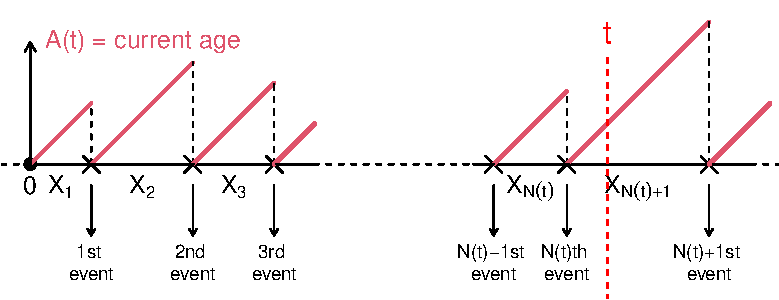
\includegraphics[width=\textwidth]{L17_CurrentAge.pdf}
\end{center}
What is the long-run average of age
$\displaystyle\lim_{t\to\infty}\frac{\int_0^tA(s)ds}{t}?$
\end{frame}
% ----------------------------------------------------------------------
\begin{frame}{Example 7.19 Residual Life of a Renewal Process}
Consider the {\bf residual life} or {\bf excess} of the item in use at time $t$
$$Y(t) = S_{N(t)+1}- t.$$
\begin{center}
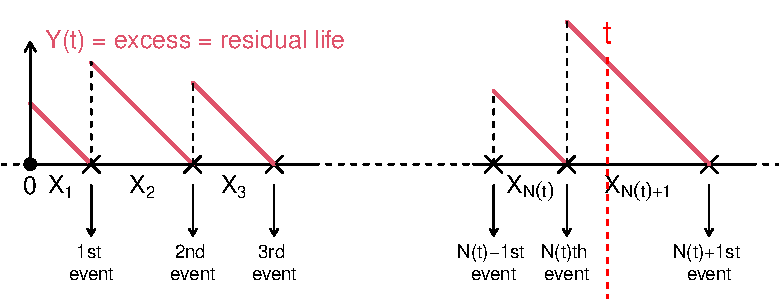
\includegraphics[width=\textwidth]{L17_ResidualLife.pdf}
\end{center}
What is the long-run average of residual life
$$
\lim_{t\to\infty}\frac{\int_0^tY(s)ds}{t}?
$$
\end{frame}
% ----------------------------------------------------------------------
\begin{frame}{Example 7.18 Age of a Reward Renewal Process (Cont'd)}
Observe that $\int_0^tA(s)ds$ is the area of the shaded regions below.
\begin{center}
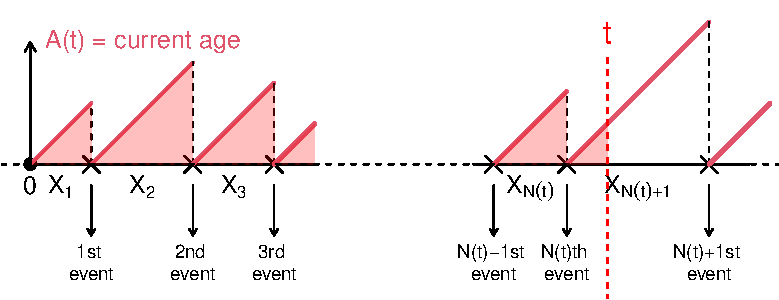
\includegraphics[width=\textwidth]{L17_CurrentAgeArea.pdf}
\end{center}
$$
\Sum_{i=1}^{N(t)}\frac{X_i^2}{2} \le \int_0^tA(s)ds<\Sum_{i=1}^{N(t)+1}\frac{X_i^2}{2}
$$
Observe that $\sum_{i=1}^{N(t)}\frac{X_i^2}{2}$
is a renewal reward process $R(t) =\sum_{i=1}^{N(t)}R_i$ with reward
$R_i= X_i^2/2$.

\end{frame}
% ----------------------------------------------------------------------
\begin{frame}{Example 7.18 Current Age (Cont'd)}
Since
$$R(t)\le \int_0^tA(s)ds <R(t)+\frac{X_{N(t)+1}^2}{2},$$
and
\begin{align*}
\frac{X_{N(t)+1}^2}{2t}\to 0\quad\text{as }t\to\infty.
\end{align*}
by Proposition 7.3, the long-run average age of the item in use is
$$
\frac{\int_0^tA(s)ds}{t}
= \lim_{t\to\infty}\dfrac{R(t)}{t}
=\dfrac{\E[R_1]}{\E[X_1]}=\frac{\E[X_1^2]}{2\E[X_1]}.
$$
\end{frame}
% ----------------------------------------------------------------------
\begin{frame}{Example 7.19 Residual Life (Cont'd)}
Similarly, for the residual life, $\int_0^tY(s)ds$ is the area of the shaded regions below.
\begin{center}
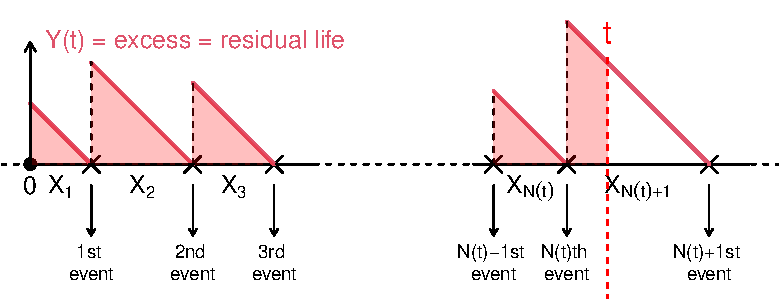
\includegraphics[width=\textwidth]{L17_ResidualLifeArea.pdf}
\end{center}
$$
\Sum_{i=1}^{N(t)}\frac{X_i^2}{2} \le \int_0^tY(s)ds<\Sum_{i=1}^{N(t)+1}\frac{X_i^2}{2}
$$
By the same argument, the long-run average of residual life of the item in
use is
$$
\frac{\int_0^tY(s)ds}{t}
= \lim_{t\to\infty}\dfrac{R(t)}{t}
=\dfrac{\E[R_1]}{\E[X_1]}=\frac{\E[X_1^2]}{2\E[X_1]}.
$$
\end{frame}
% ----------------------------------------------------------------------
\begin{frame}{7.5.1 ~Alternating Renewal Processes}
Considers a system that can be in one of two states: {\bf ON} or {\bf OFF}.
Initially it is ON, and remains ON for a time $Z_1$; it then goes OFF
and remains OFF for a time $Y_1$. It then goes ON for a time $Z_2$;
then OFF for a time $Y_2$; then on, and so on. Suppose
\begin{itemize}
\item $(Z_k,Y_k)$ are i.i.d random vectors, though $Z_k$ and $Y_k$ might depend on each other
\item $Y_k$, $Z_k$ are non-negative with finite means.
\end{itemize}
Then a renewal process $\{N(t),t \ge 0\}$ with interarrival times
$$X_k= Z_k+ Y_k,\qquad k \ge 1$$
is called an \structure{\em alternating renewal process}.
Let
$$
U(t) =
\begin{cases}
1 & \text{if the system is ON at time }t\\
0 & \text{otherwise}
\end{cases}
$$
{\bf Q}: What is the long-run proportion of time that the system is ON?
$$
\lim_{t\to\infty} \frac{\int_0^t U(s)ds}{t}?
$$
\end{frame}
% ----------------------------------------------------------------------
\begin{frame}{Alternating Renewal Processes (Cont'd)}
An alternating renewal process can be regarded as a renewal reward process with reward $R_i= Z_i$,
$$
R(t) = \Sum_{i=1}^{N(t)}Z_i
$$
Then
$$
R(t)\le \int_0^t U(s)ds < R(t) + Z_{N(t)+1}
$$
By Proposition 7.3, with probability 1,
$$
\lim_{t\to\infty} \frac{R(t)}{t}=\frac{\E[Z_1]}{E[X_1]}=\frac{\E[Z_1]}{\E[Z_1] + \E[Y_1]}
$$
and hence
$$
\lim_{t\to\infty} \frac{\int_0^t U(s)ds}{t}=\lim_{t\to\infty} \frac{R(t)}{t}
=\frac{\E[Z_1]}{\E[Z_1] + \E[Y_1]}=\frac{\E[\text{ON}]}{\E[\text{ON}] + \E[\text{OFF}]}.
$$
\end{frame}
% ----------------------------------------------------------------------
\begin{frame}{Definition: Lattice Distribution}
A random variable $X$ is said to have a {\bf lattice} distribution if there is
an $h > 0$ for which
$$\Sum_{k=-\infty}^{\infty} P(X = kh) = 1,$$
i.e., $X$ is lattice if it only takes on integral multiples of some nonnegative number $h.$
The largest $h$ having this property is called the \structure{\em period} of $X$.\medskip

{\bf Examples}.
\begin{itemize}
\item Continuous distributions, mixtures of discrete and continuous distributions are both non-lattice.
\item Integer-valued random variables are lattice, e.g., Poisson, binomial
\item A lattice distribution must be discrete, but a discrete distribution may not be lattice,
e.g., if

\vspace{-12pt}
$$\p(X=1/n)=1/2^n,\quad n=1,2,3,\ldots$$
then $X$ is discrete but non-lattice because
we cannot find an $h>0$ such that all $1/n$'s are all multiples of $h$.
\end{itemize}
\end{frame}
% ----------------------------------------------------------------------
\begin{frame}
%Remark: If $X_i$'s are i.i.d with a common lattice distribution, then
%$$S_n= X_1+ \ldots + X_n$$
%also has a lattice distribution for all $n.$
{\bf Theorem} If the interarrival distribution is non-lattice, then
$$\lim_{t\to\infty}\p(\text{ON at time }t)
= \lim_{t\to\infty}\p(U(t) = 1) = \frac{\E[Z_1]}{\E[Z_1] + \E[Y_1]}$$
\medskip
{\bf Remark}. If interarrival distribution is lattice, $\lim_{t\to\infty}\p(U(t) = 1)$ may not exist.


\end{frame}
% ----------------------------------------------------------------------
\begin{frame}{Exercise 7.39}
\begin{itemize}
\item Two machines work independently, each functions for an exponential
time with rate $\lambda$ and then fails
\item A single repairmen. All repair times are independent with
distribution function $G$
\item If the repairmen is free when a machine fails, he will begin
repairing that machine immediately; Otherwise, that
machine must wait until the other machine has been repaired.
\item Once repaired, a machine is as good as a new one.
\item What proportion of time is the repairmen idle?
\end{itemize}
{\em Solution.}
\begin{itemize}
\item ON when the repairmen is idle, OFF when busy
\item length of ON (idle)  time: $Z \sim Exp(2\lambda)$, $\E[Z] = 1/(2\lambda)$
\item length of OFF (busy) time $Y$; want to find $\E[Y]$
\end{itemize}
\end{frame}
% ----------------------------------------------------------------------
\begin{frame}{Exercise 7.39~ Solutions}
\begin{itemize}
\item $T =$ length of time to repair the first failing machine $\sim G$
\item $U =$ the time the working machine can function after the first
machine failed. By the memoryless property, $U \sim Exp(\lambda)$
\item Note that

\vspace{-26pt}\begin{align*}
Y &=
\begin{cases}
T    & \text{if } U > T\\[-3pt]
T+Y' & \text{if } U < T
\end{cases}\\
&=T+Y'\mathbf{1}_{\{U<T\}}
\end{align*}
where $Y'$ is the time the repairmen remains busy after the
first failing machine is fixed. Note $Y'$ is independent of
$T$ and $U$, and has the same distribution as $Y$. Thus
$$
\E[Y] = \E[T] + \E[Y]\p(T > U)\;\Rightarrow\; \E[Y] = \frac{\E[T]}{\p(T < U)}
$$
%\item Since $U \sim Exp(\lambda)$,
%$$\p(T < U) = \int_0^{\infty} \p(U>t)dG(t)=\int_0^{\infty} e^{-\lambda t}dG(t)$$
\item long-run proportion of ON (idle) time $$\dfrac{\E[Z]}{\E[Z] + \E[Y]}
=\dfrac{1/(2\lambda)}{1/(2\lambda) + \E[Y]}$$
\end{itemize}
\end{frame}
% ----------------------------------------------------------------------
\begin{frame}{Example 7.23 \& 7.24}
Let $\{N(t),\;t \geq 0\}$ be a renewal process with i.i.d. interarrival times
$X_i$, $i = 1,2,\ldots$, where $\mu = \E[X_i]$ and $F(x) = P(X_i\le x)$.
Consider the {\bf current age} of the item in use at time $t$
$$A(t) = t - S_{N(t)},$$
and the {\bf residual life} of the item in use at time $t$
$$Y(t) = S_{N(t)+1}- t.$$

{\bf Proposition}. The long-run proportion of time that $A(t) \le x$ is the
same as the long-run proportion of time that $Y(t) \le x$, and is equal to
$$
F_e(x) =\frac{1}{\mu}\int_0^x(1 - F(u))du.
$$
Furthermore, if $F$ is non-lattice, then
$$\lim_{t\to\infty}\p(A(t)\le x) = \lim_{t\to\infty}\p(Y(t)\le x) = F_e(x).$$
\end{frame}
% ----------------------------------------------------------------------
\begin{frame}{Example 7.23 Current Age(Con'd)}
\begin{center}
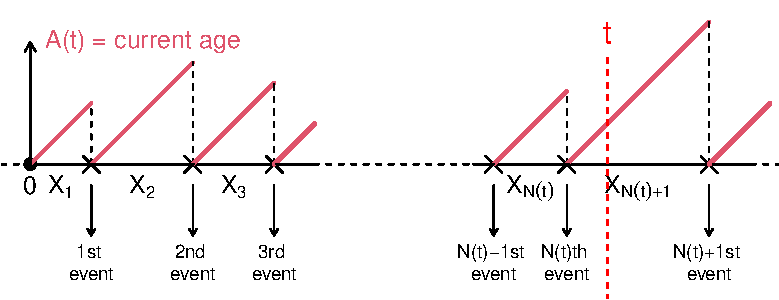
\includegraphics[width=0.9\textwidth, trim=0 45 0 0, clip]{L17_CurrentAge.pdf}
\end{center}
\begin{itemize}
\item let's say the system is ON at time $t$ if $A(t) \le x$
\item length of ON time $Y_i= \min(X_i,x)$
\begin{align*}
\E[Y_i] = \E[\min(X_i,x)] &= \int_0^{\infty}\p(\min(X_i,x) > u)du\\
&=\int_0^x (1 - F(u))du
\end{align*}
\item length of a cycle $= X_i$, $\E[\text{ON}] + \E[\text{OFF}] = \E[X_i] = \mu$
\item long-run proportion of time that $A(t) \le x$ is
$$\frac{\E[\text{ON}]}{\E[\text{ON}] + \E[\text{OFF}]}=\frac{1}{\mu}\int_0^x (1 - F(u))du$$
\end{itemize}
\end{frame}
% ----------------------------------------------------------------------
\begin{frame}{Example 7.24 Residual Life (Con'd)}
\begin{center}
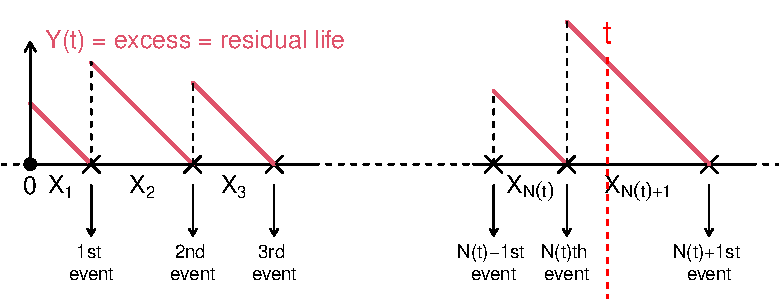
\includegraphics[width=0.9\textwidth, trim=0 45 0 0, clip]{L17_ResidualLife.pdf}
\end{center}
\begin{itemize}
\item let's say the system is OFF at time $t$ if $Y(t) \le x$
\item length of OFF time $Z_i= \min(X_i,x)$
$$\E[Z_i] = \E[\min(X_i,x)] =\int_0^x (1 - F(u))du$$
\item length of a cycle $= X_i$, $\E[\text{ON}] + \E[\text{OFF}] = \E[X_i] = \mu$
\item long-run proportion of time that $Y(t) \le x$ is
$$\frac{\E[\text{OFF}]}{\E[\text{ON}] + \E[\text{OFF}]}=\frac{1}{\mu}\int_0^x (1 - F(u))du$$
\end{itemize}
\underline{Remark}: The ON time in Example 7.23 is not the same as the
ON time in Example 7.24
\end{frame}
% ----------------------------------------------------------------------
%\begin{frame}%{About $F_e$}
%The density and $k$th moment of the distribution $F_e$ is
%$$
%f_e(x) =\frac{1}{\mu}(1 - F(x)),\quad\text{and}\quad
%\int_0^{\infty}x^k f_e(x)dx =\frac{\E[X^{k+1}]}{(k + 1)\E[X]}
%$$
%where $X$ is an interarrival time.
%
%Recall that
%$$\frac{m(t)}{t}=\frac{1}{\mu}-\frac{1}{t}+\frac{\E[Y(t)]}{t\mu}$$
%If $F$ is non-lattice, since the limiting distribution of $Y(t)$ is $F_e$, we
%have
%$$\lim_{t\to\infty}=\E[Y(t)] =\frac{\mu^2+ \sigma^2}{2\mu}$$
%Thus
%$$
%m(t) =\frac{t}{\mu}- 1 +\frac{\mu^2+ \sigma^2}{2\mu^2}+ o(t)
%=\frac{t}{\mu}+\frac{\sigma^2-\mu^2}{2\mu^2}+ o(t)
%$$
%\end{frame}
% ----------------------------------------------------------------------
\end{document}
\begin{frame}
\end{frame}
% ----------------------------------------------------------------------
\begin{frame}{7.5\; Regenerative Processes}
A \structure{\bf regenerative process} a stochastic process $\{X(t), t \ge 0\}$ having
the property that there exist time points $T_1$ at which the process (probabilistically)
restarts itself. That is
$$
\{X(t+T_1), t \ge 0\}\sim\{X(t), t \ge 0\}
$$
Note that this property implies the existence of further times $T_2$, $T_3,\ldots$, having the same property as $T_1$, and it follows that $T_1$, $T_2,\ldots$, constitute the arrival times of a renewal process.\bigskip

{\bf Example}. A recurrent Markov chain is regenerative, and $T_1$ represents the time of the first
transition into the initial state.
\end{frame}
% ----------------------------------------------------------------------
\begin{frame}{Markov Chain and Renewal Process}
Given a Markov chain $\{X_n, n\ge 0\}$, $X_0=i$. Let
\begin{align*}
N_i(t)&=\Sum_{0\le n\le t}\mathbf{1}_{\{X_n=i\}}\\
&=\mbox{number of times the chain visits state $i$ by time $t$}
\end{align*}
Note that $\{N_i(t), t\ge 0\}$ is a renewal process
where the interarrival times $T(i)$ are the number of steps between consecutive visits to state $i$.\bigskip

In either cases, we have the Elementary Renewal Theorem (Thm 7.1)
$$
\lim_{t\to\infty}\frac{m_i(t)}{t}=\frac{1}{\E(T(i))}
$$
where $m_i(t)=\E[N(t)]=\Sum_{0\le n\le t}P(X_n=i)=\Sum_{0\le n\le t}P^{(n)}_{ii}$
\end{frame}
% ----------------------------------------------------------------------
\begin{frame}{Markov Chain and Renewal Process (Cont'd)}
At every cycle, the renewal process is ON for one unit of time after every visits to state $i$.
So length of ON time in a cycle is fixed at $1$.
By Proposition 7.4, it follows that
$$
\mbox{the long-run proportion of time in state }i=\frac{1}{\E[\mbox{cycle time}]}=\frac{1}{\E[T_i]}
$$
\end{frame}
% ----------------------------------------------------------------------
